\documentclass[12pt]{article}
\usepackage[margin=1in]{geometry}
\usepackage{listings}
\usepackage{graphicx}
\usepackage{float}
\usepackage{color} %red, green, blue, yellow, cyan, magenta, black, white
\definecolor{mygreen}{RGB}{28,172,0} % color values Red, Green, Blue
\definecolor{mylilas}{RGB}{170,55,241}

\setlength{\parskip}{1em}

\lstset{language=Matlab,%
    %basicstyle=\color{red},
    breaklines=true,%
    morekeywords={matlab2tikz},
    keywordstyle=\color{blue},%
    morekeywords=[2]{1}, keywordstyle=[2]{\color{black}},
    identifierstyle=\color{black},%
    stringstyle=\color{mylilas},
    commentstyle=\color{mygreen},%
    showstringspaces=false,%without this there will be a symbol in the places where there is a space
    numbers=left,%
    numberstyle={\tiny \color{black}},% size of the numbers
    numbersep=9pt, % this defines how far the numbers are from the text
    emph=[1]{for,end,break},emphstyle=[1]\color{red}, %some words to emphasise
    %emph=[2]{word1,word2}, emphstyle=[2]{style},    
}


\title{Assignment 2, COMP4702}
\author{Roy Portas, 43560846}
\date{\today}

\begin{document}

\begin{titlepage}
    \maketitle
\end{titlepage}

\section*{Question 4.2}

\lstinputlisting[language=Matlab]{../../pracs/week5/q2.m}

\section*{Question 4.3}

The values 1.8, 3, and 5 were chosen for the lambda values, the results are outlined below.

\begin{figure}[H]
    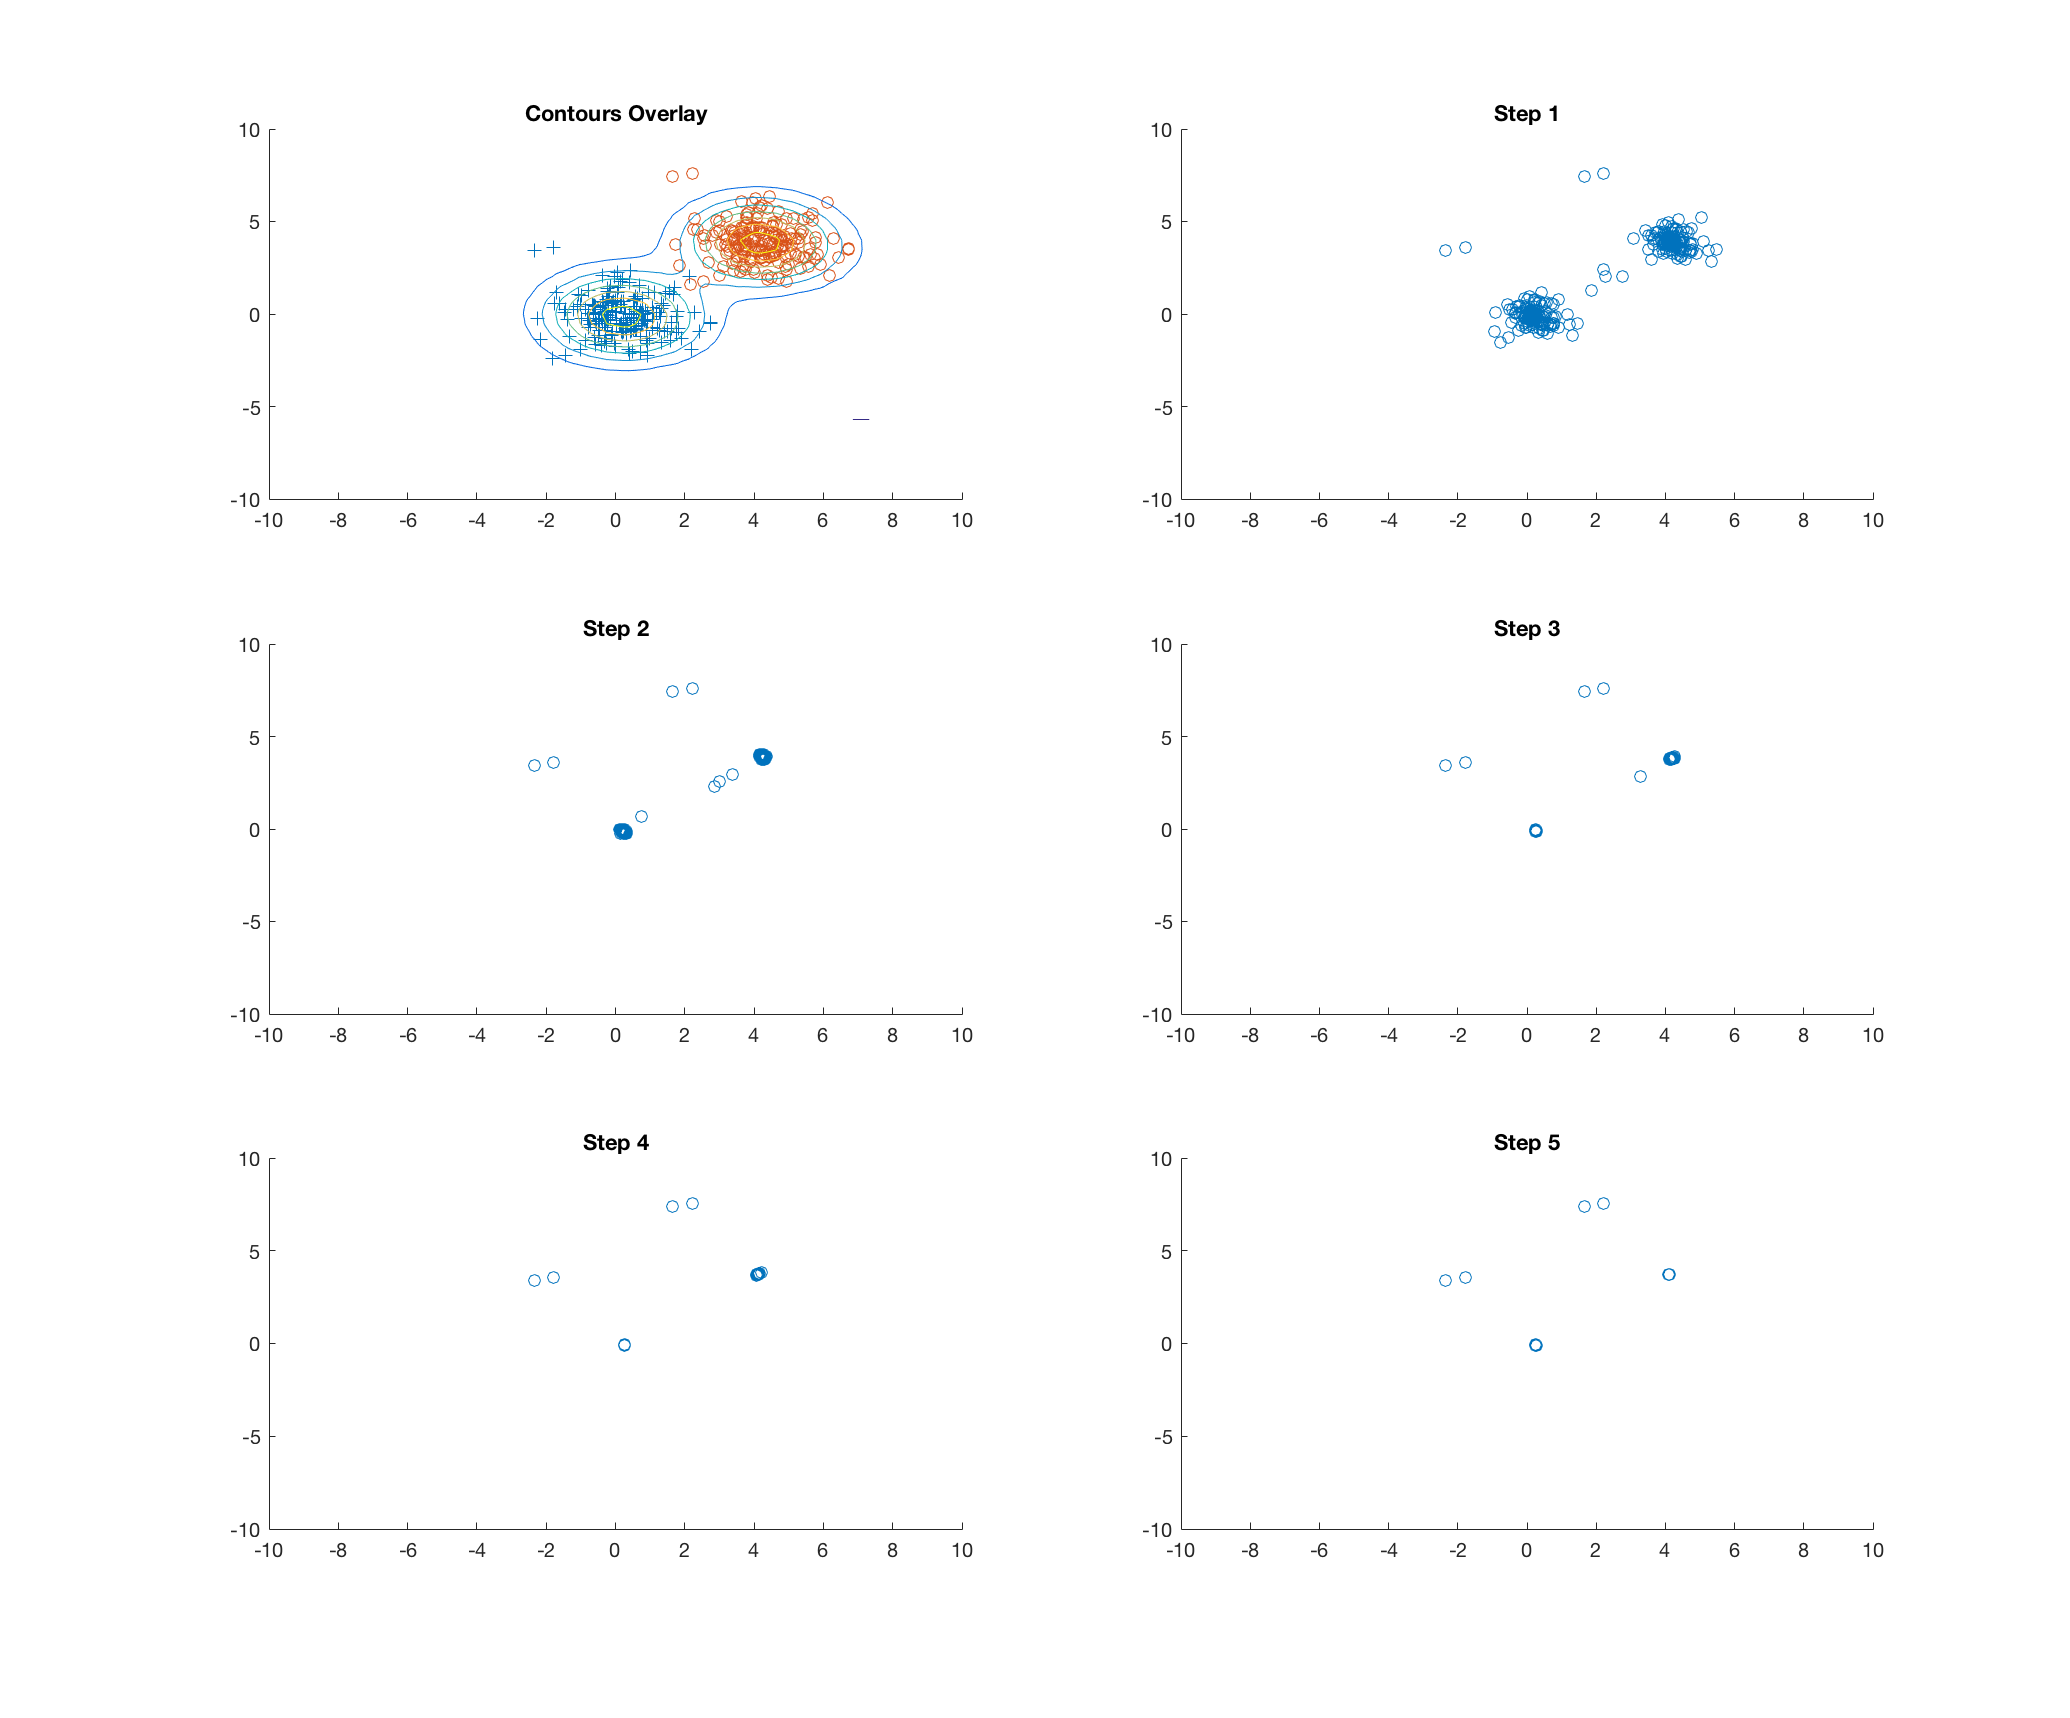
\includegraphics[width=\linewidth]{../../pracs/week5/images/q3_2class_1_8}
    \centering
    \caption{2 Classes, Lambda = 1.8}
\end{figure}

\begin{figure}[H]
    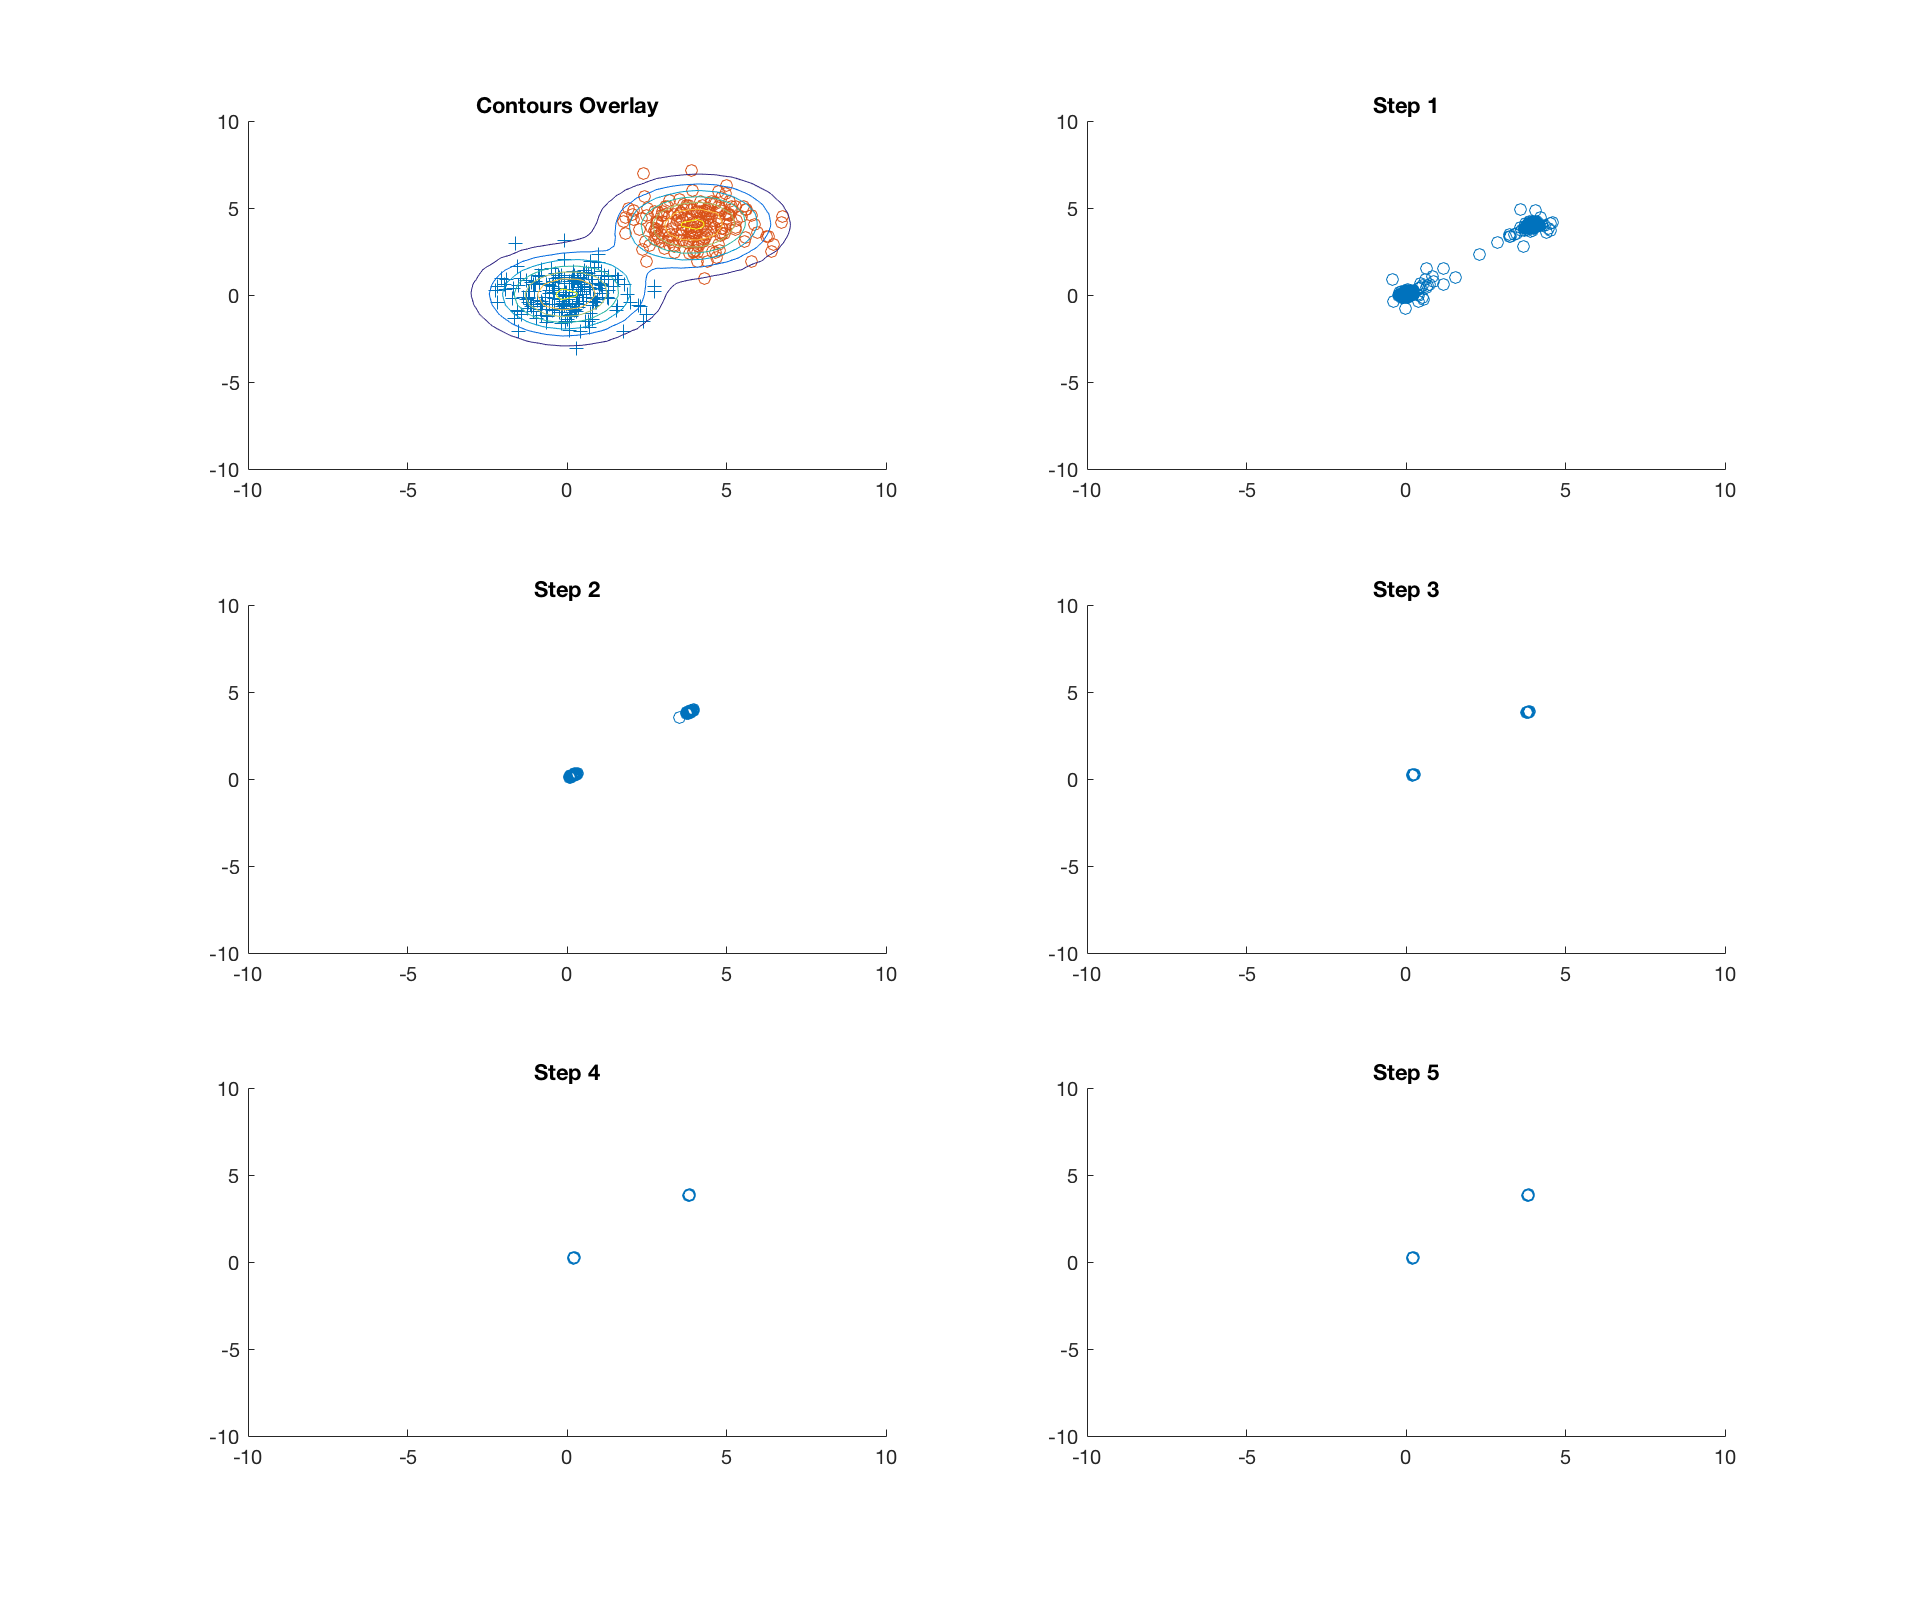
\includegraphics[width=\linewidth]{../../pracs/week5/images/q3_2class_3}
    \centering
    \caption{2 Classes, Lambda = 3}
\end{figure}

\begin{figure}[H]
    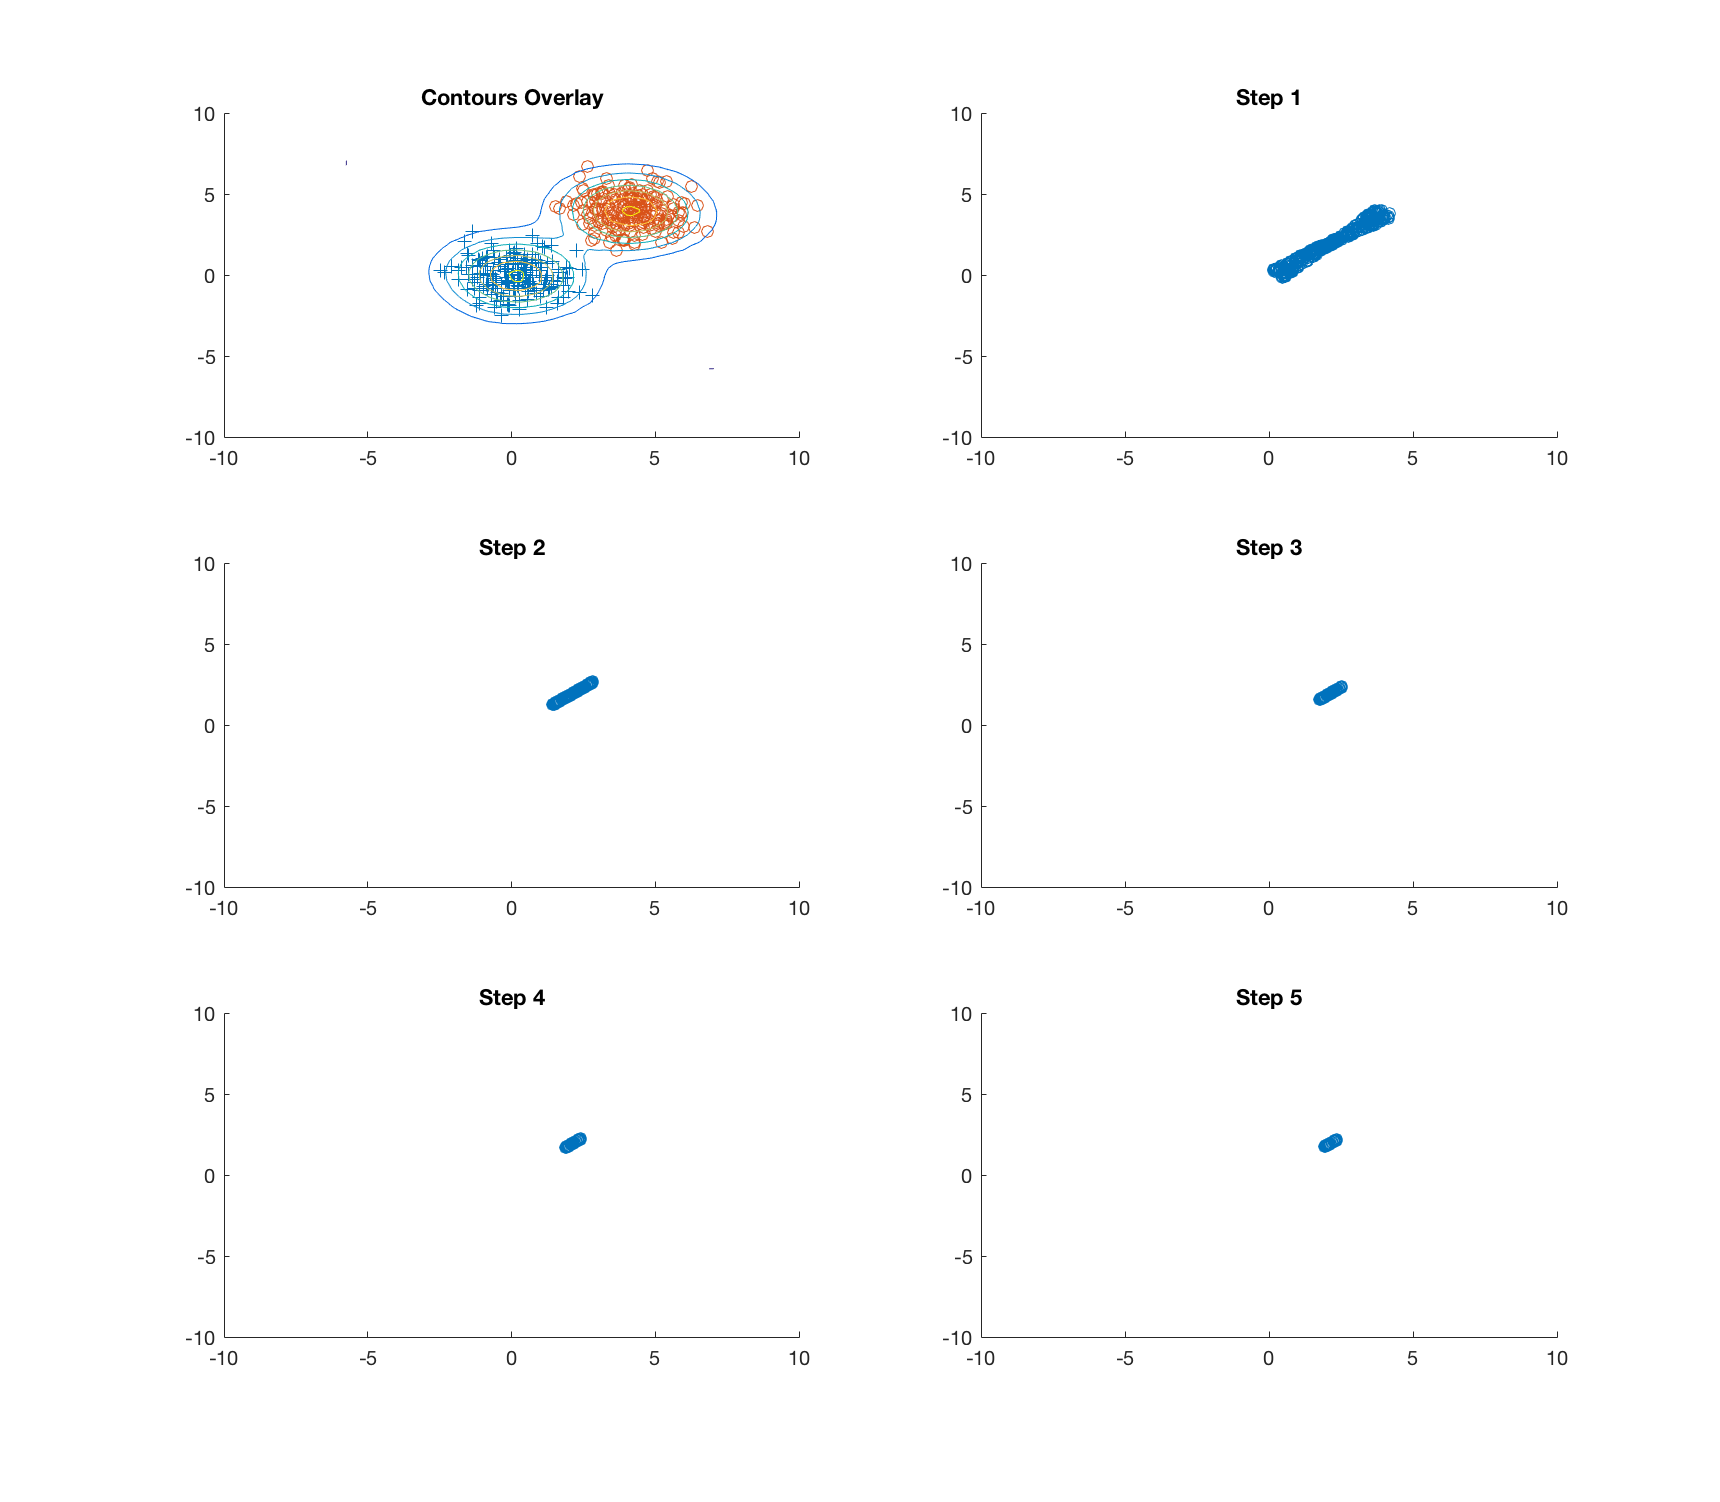
\includegraphics[width=\linewidth]{../../pracs/week5/images/q3_2class_5}
    \centering
    \caption{2 Classes, Lambda = 5}
\end{figure}

\begin{figure}[H]
    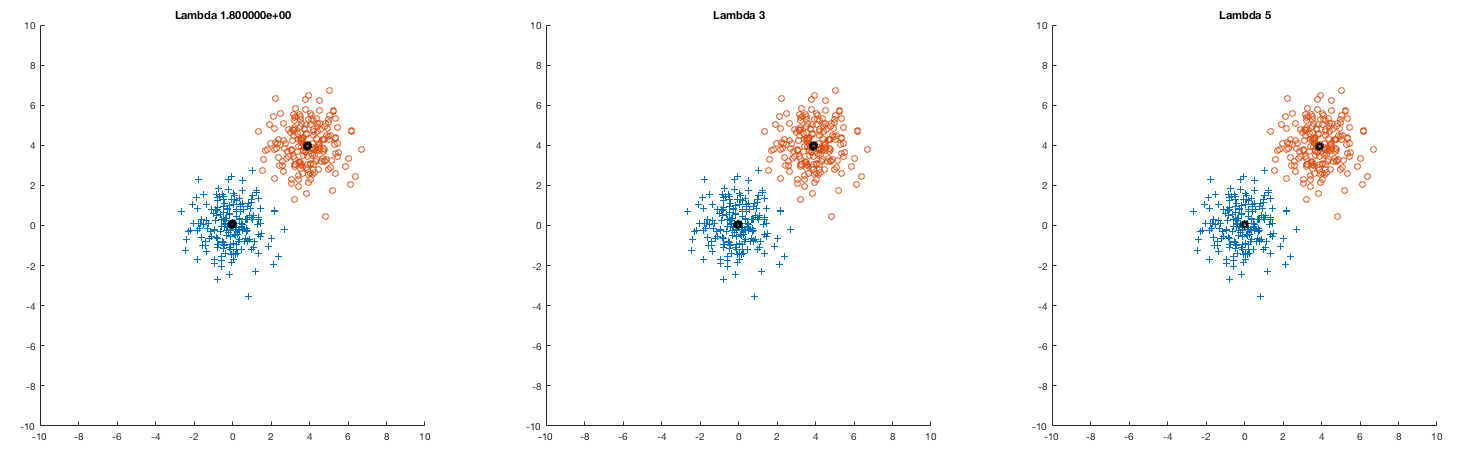
\includegraphics[width=\linewidth]{../../pracs/week5/images/q3_2class_means}
    \centering
    \caption{Cluster centres over data}
\end{figure}

For the 2 class problem, a lambda value set to 3 provided the best result. A lambda of 1.8 cause a few outliers not to shift towards the mean value.
Whereas a lambda value of 5 caused all the points to shift towards one of the means, which is not desired.
A lambda value of 3 shifted all the points to the two mean values without leaving outliers, thus is the best lambda value out of the three.

\begin{figure}[H]
    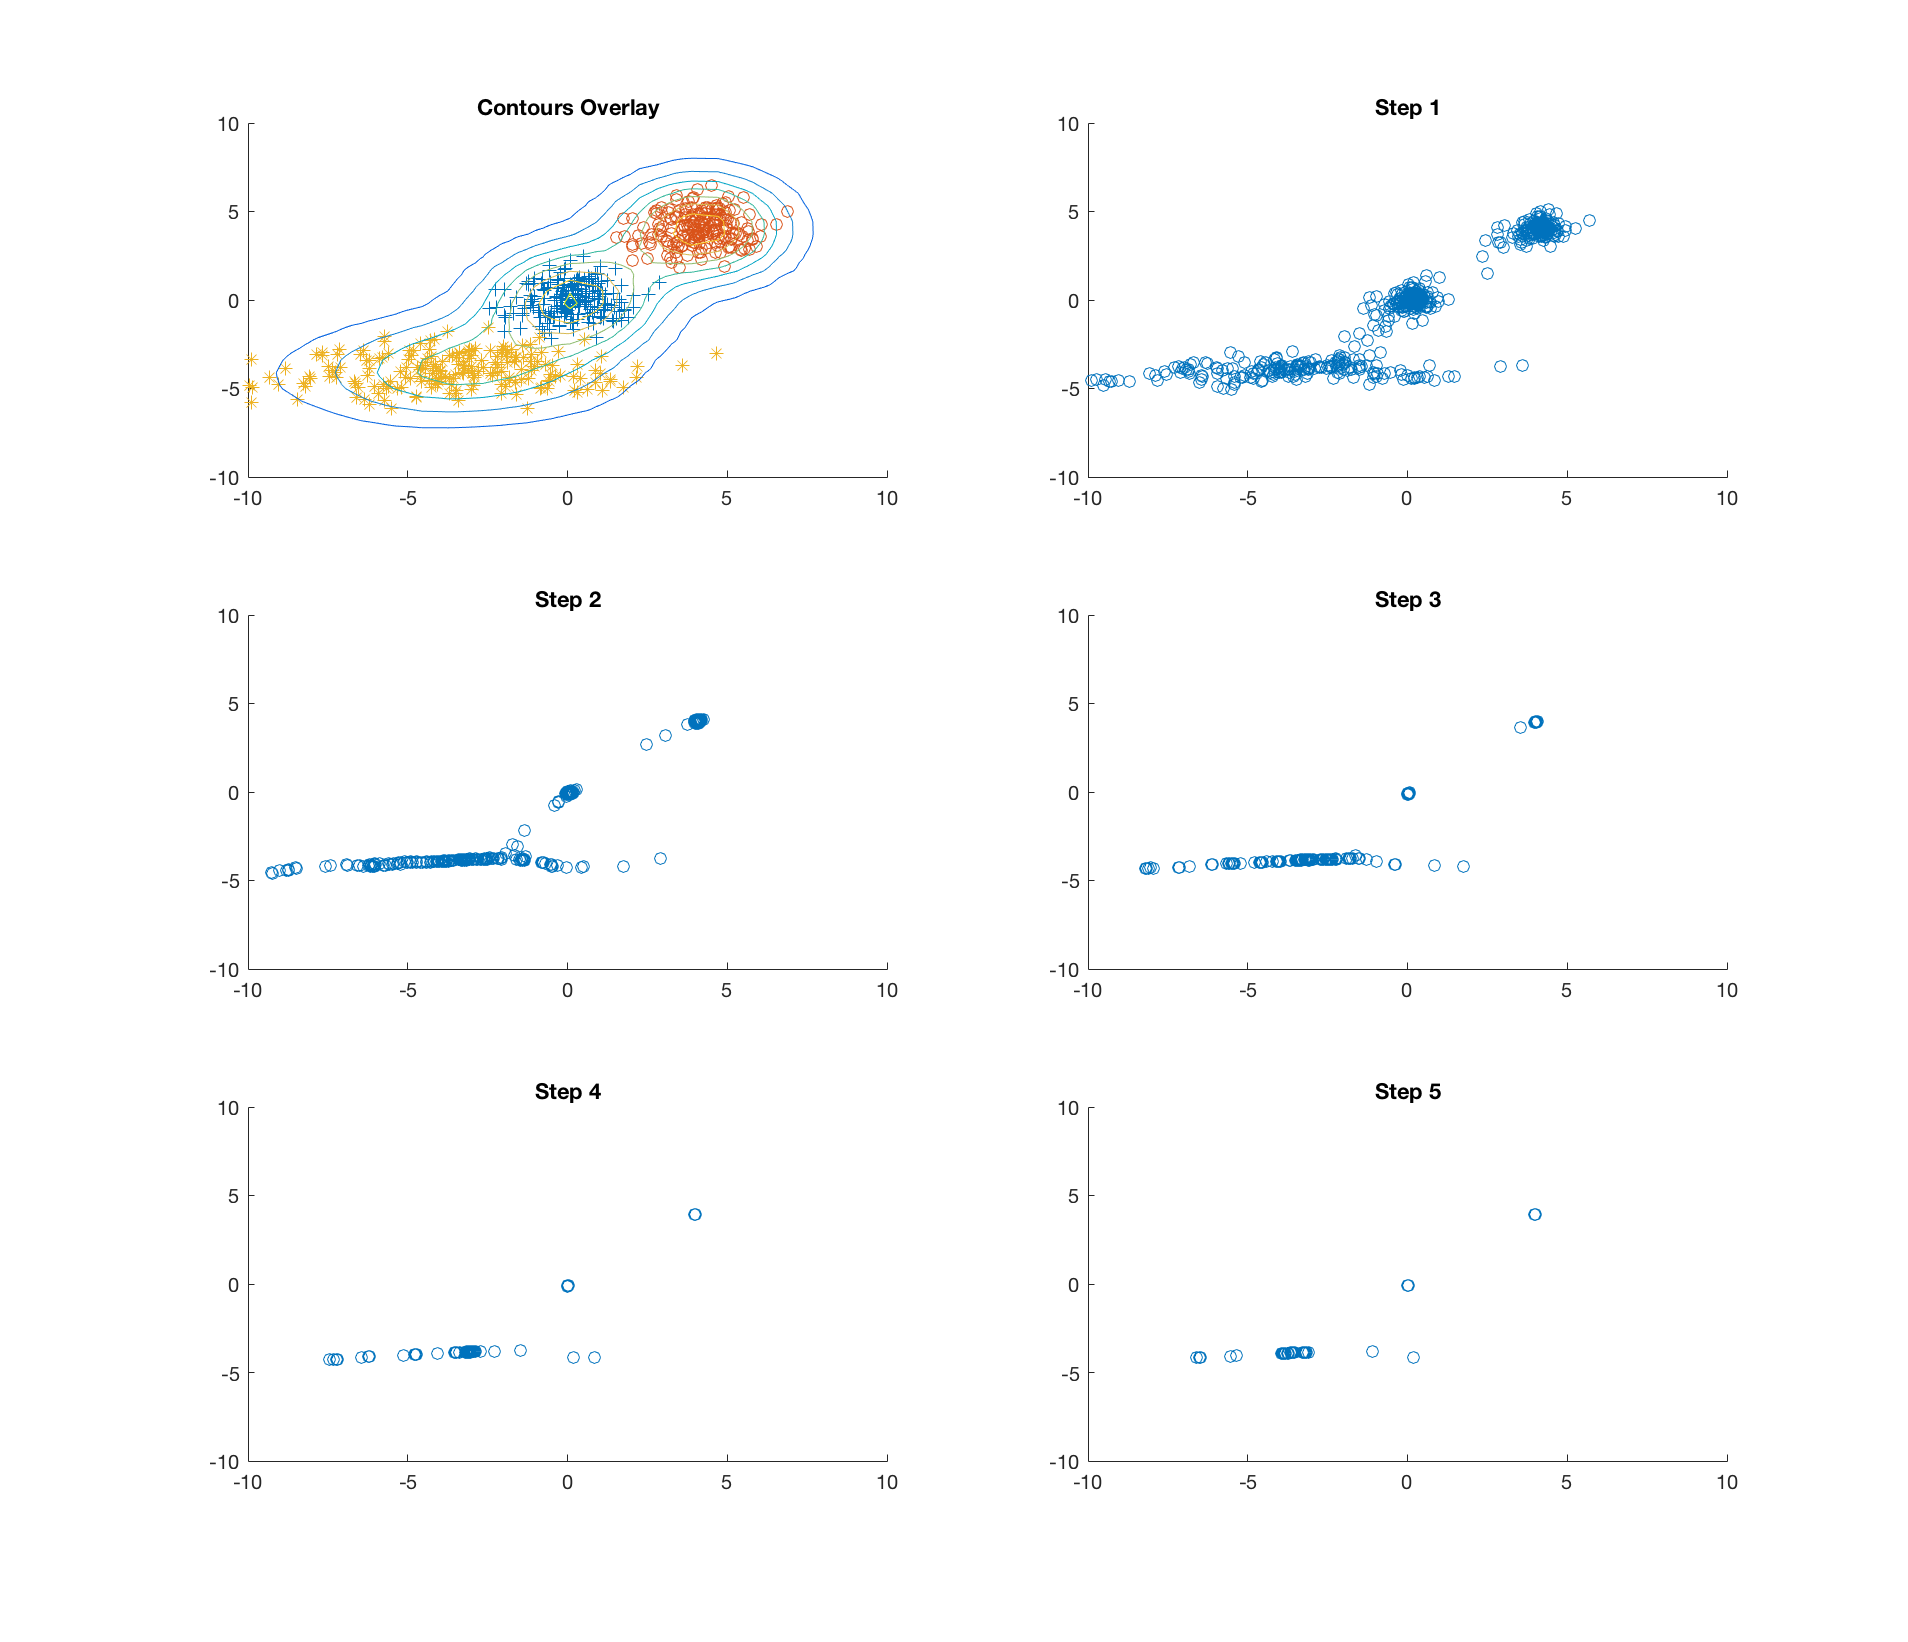
\includegraphics[width=\linewidth]{../../pracs/week5/images/q3_3class_1_8}
    \centering
    \caption{3 Classes, Lambda = 1.8}
\end{figure}

\begin{figure}[H]
    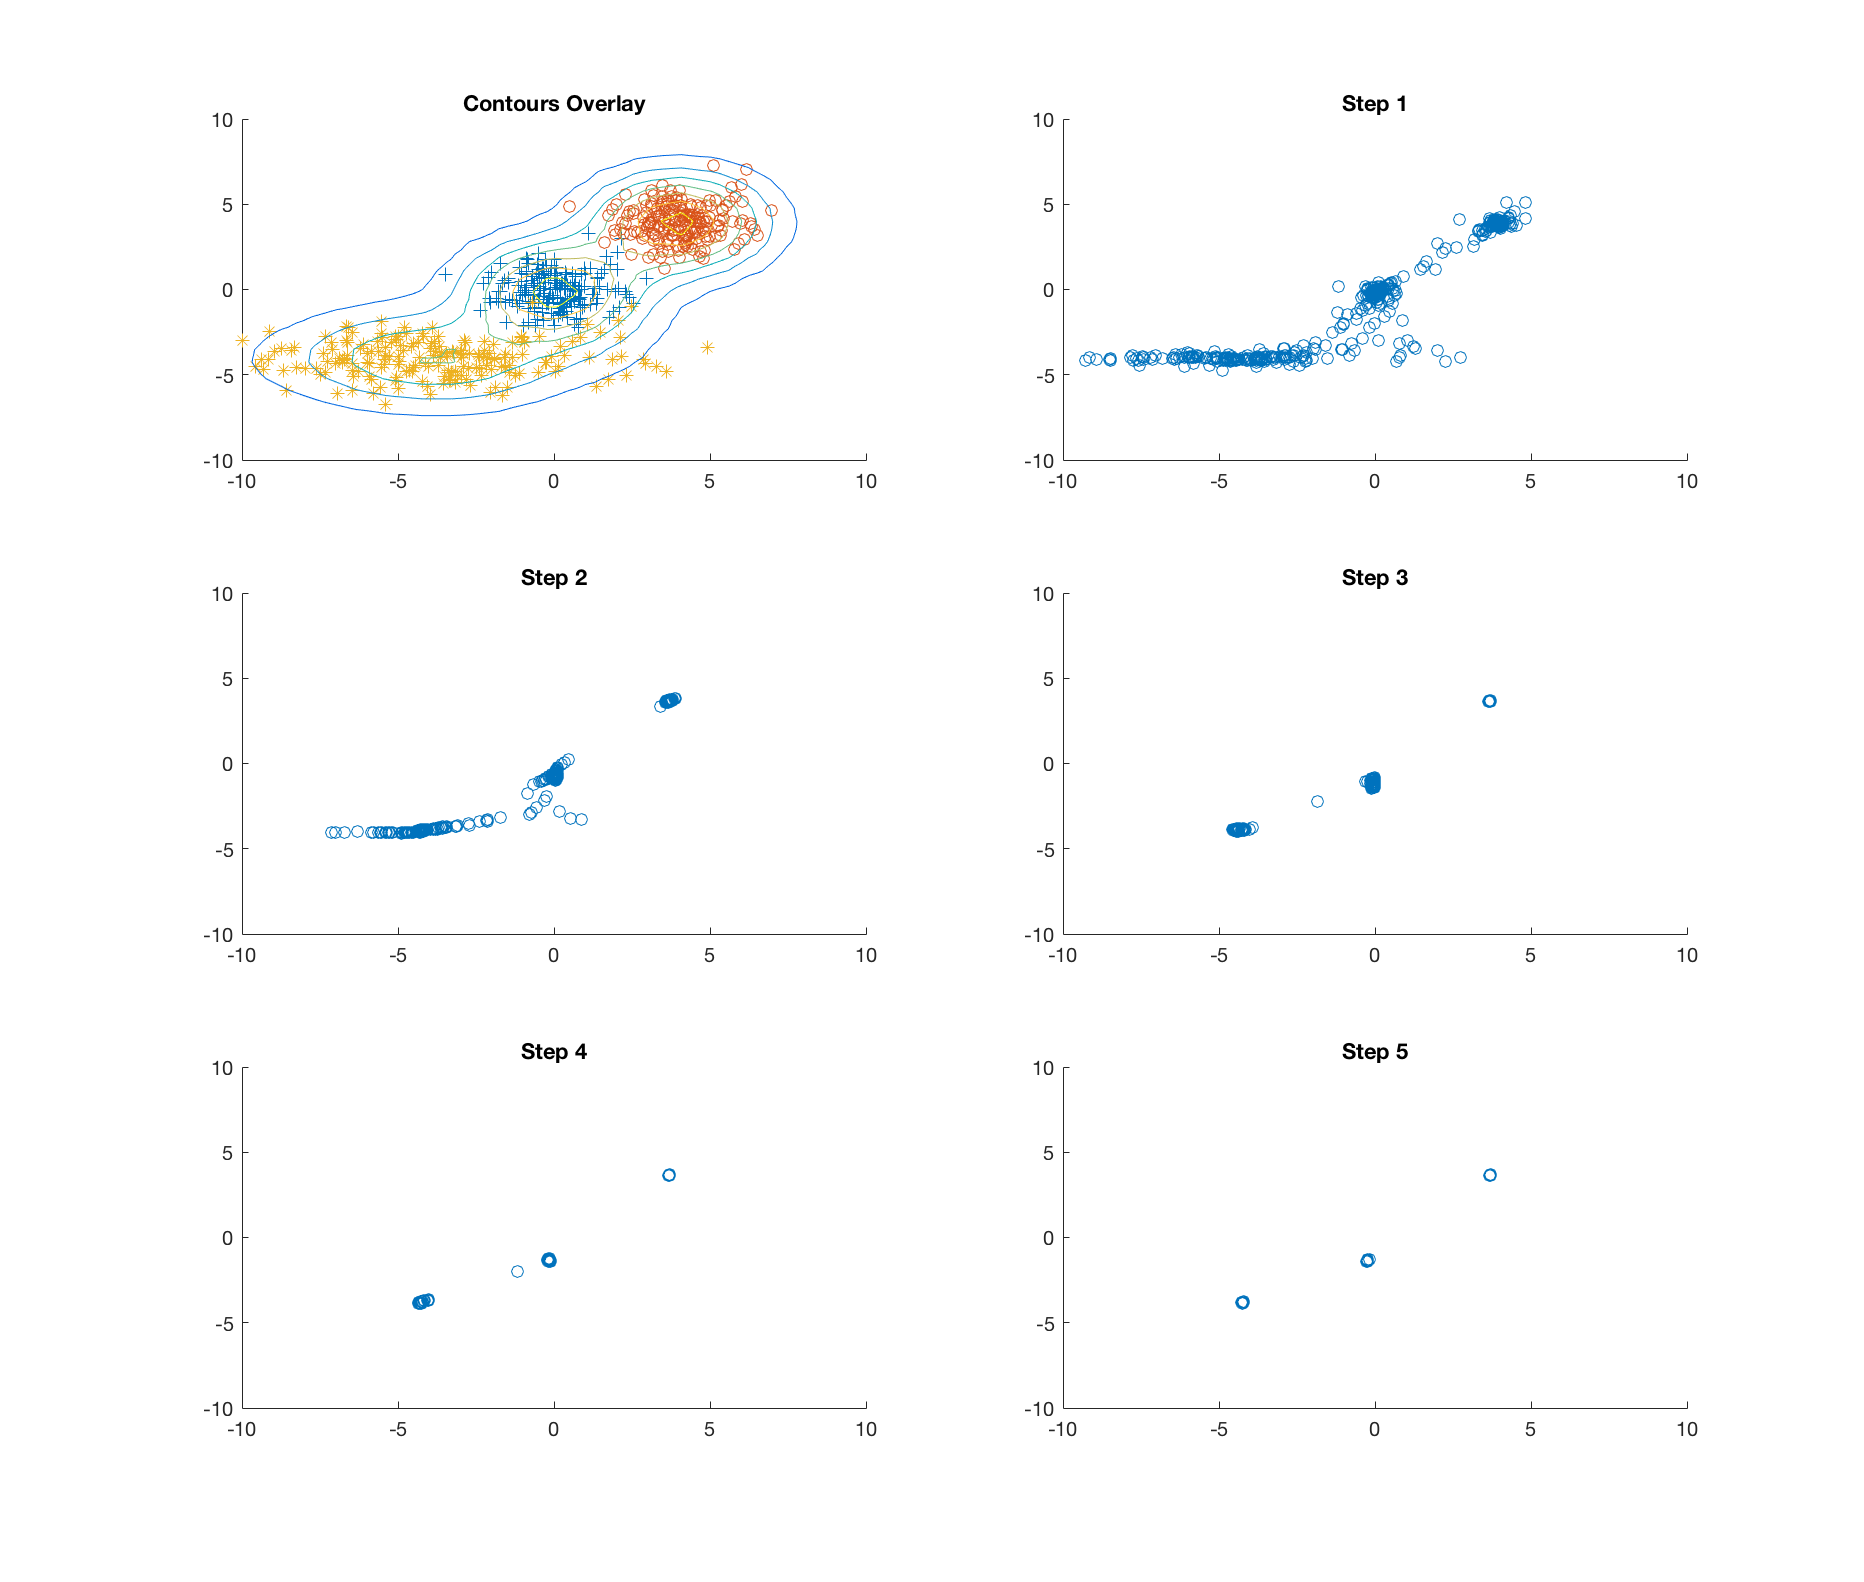
\includegraphics[width=\linewidth]{../../pracs/week5/images/q3_3class_3}
    \centering
    \caption{3 Classes, Lambda = 3}
\end{figure}

\begin{figure}[H]
    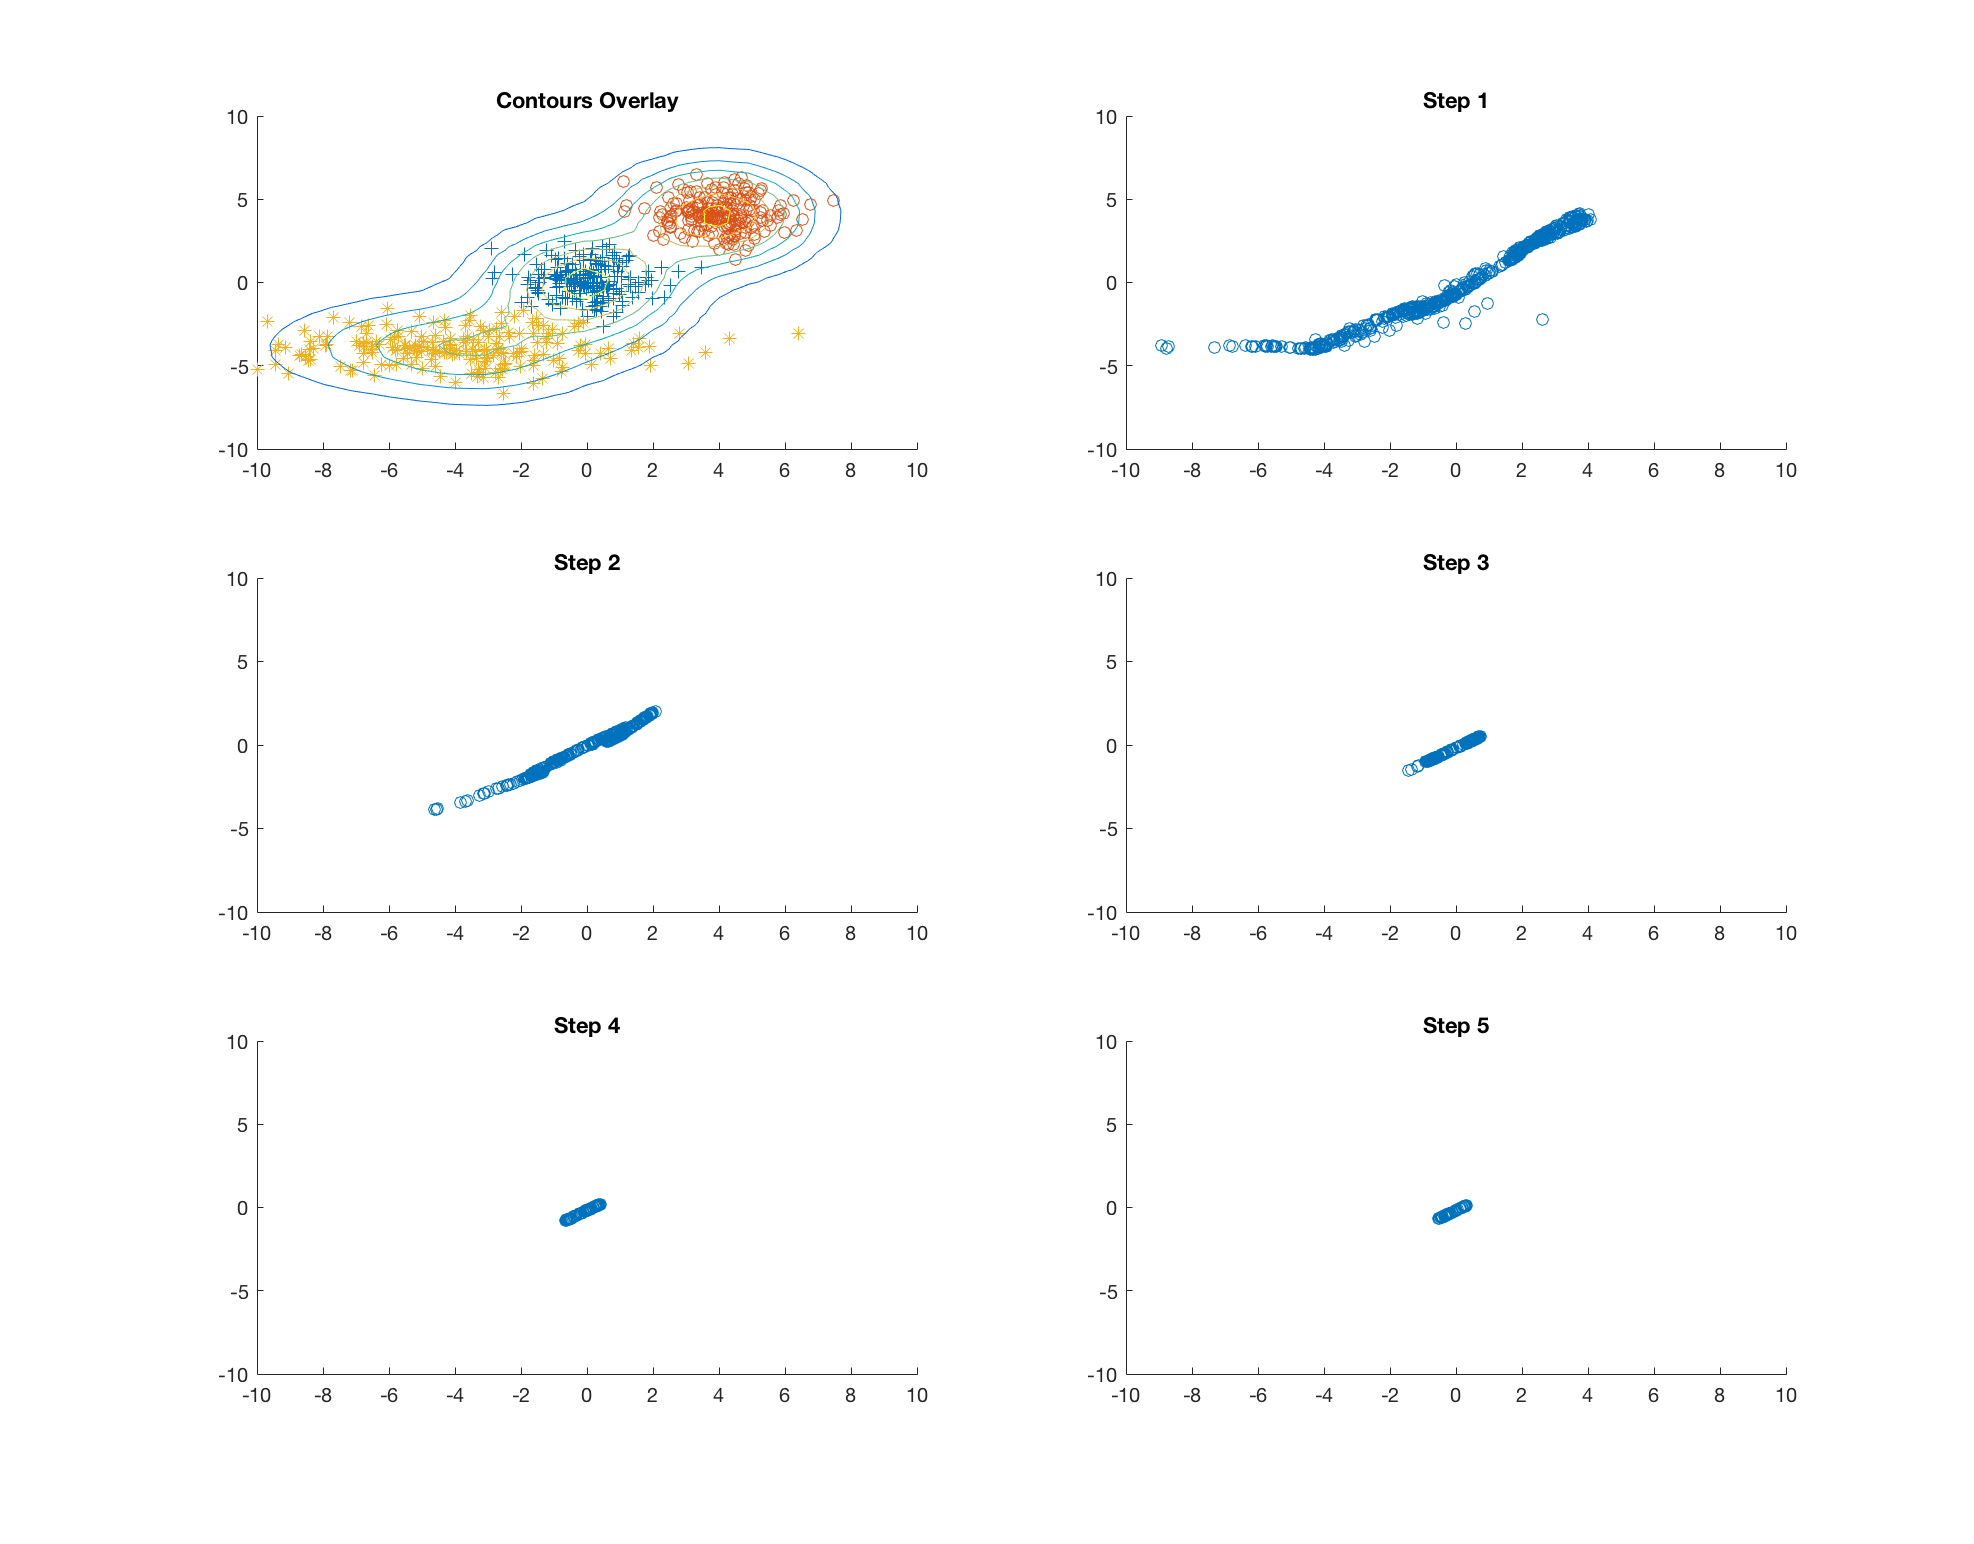
\includegraphics[width=\linewidth]{../../pracs/week5/images/q3_3class_5}
    \centering
    \caption{3 Classes, Lambda = 5}
\end{figure}

\begin{figure}[H]
    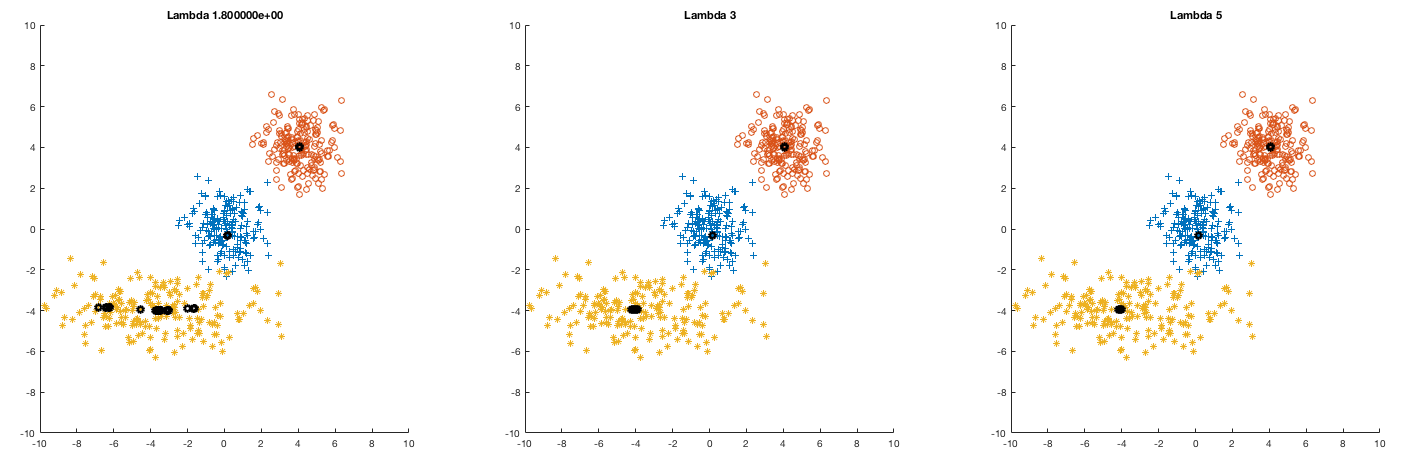
\includegraphics[width=\linewidth]{../../pracs/week5/images/q3_3class_means}
    \centering
    \caption{Cluster centres over data}
\end{figure}

The 3 class problem showed similar results with the same lambda values 1.8, 3 and 5.
Again the 1.8 lambda value failed to shift some outliers towards the mean and the 5 lambda value shifted all of them towards a single point.
The lambda value 3 correctly shifted all the points to their respective means, thus the lambda value of 3 was the best choice out of the three numbers.

\newpage
\section*{Question 5.1}

\lstinputlisting[language=Matlab]{../../pracs/week6/pca.m}

\section*{Question 5.2}

\subsection*{a}

\begin{figure}[H]
    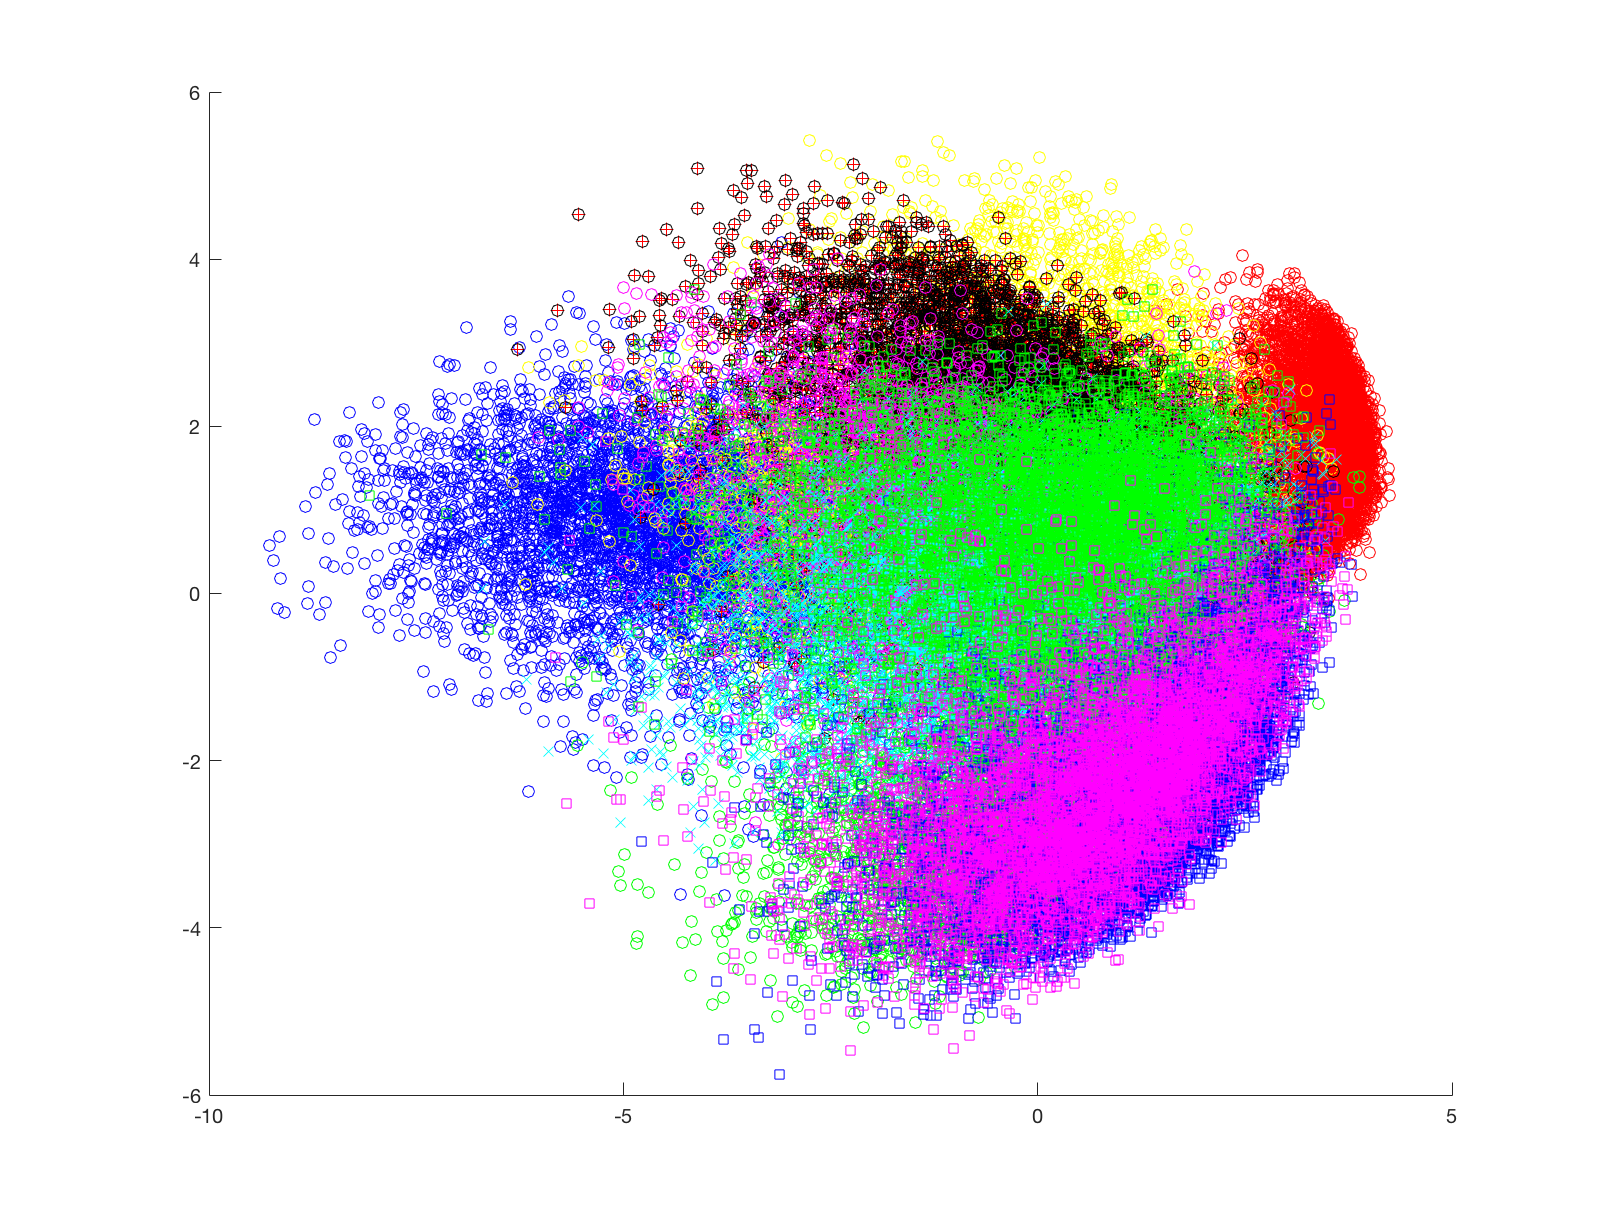
\includegraphics[width=\linewidth]{../../pracs/week6/images/q2_pca}
    \centering
    \caption{PCA on MNIST dataset}
\end{figure}

\subsection*{b}

The first principle component accounts for 9.7047\% of the data, whereas the second principle component accounts for 7.0959\% of the data.

\subsection*{c}

\begin{figure}[H]
    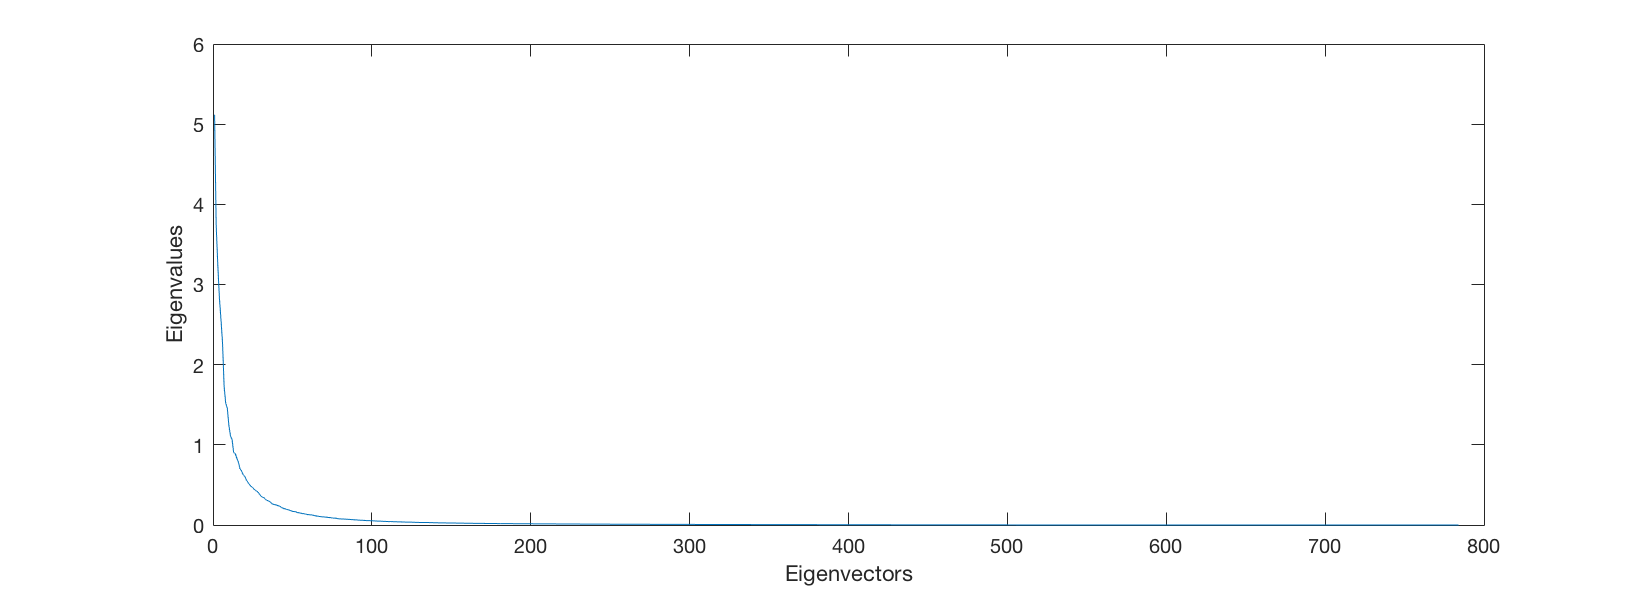
\includegraphics[width=\linewidth]{../../pracs/week6/images/scree_graph}
    \centering
    \caption{Scree Graph}
\end{figure}

\section*{Question 5.6}

\begin{figure}[H]
    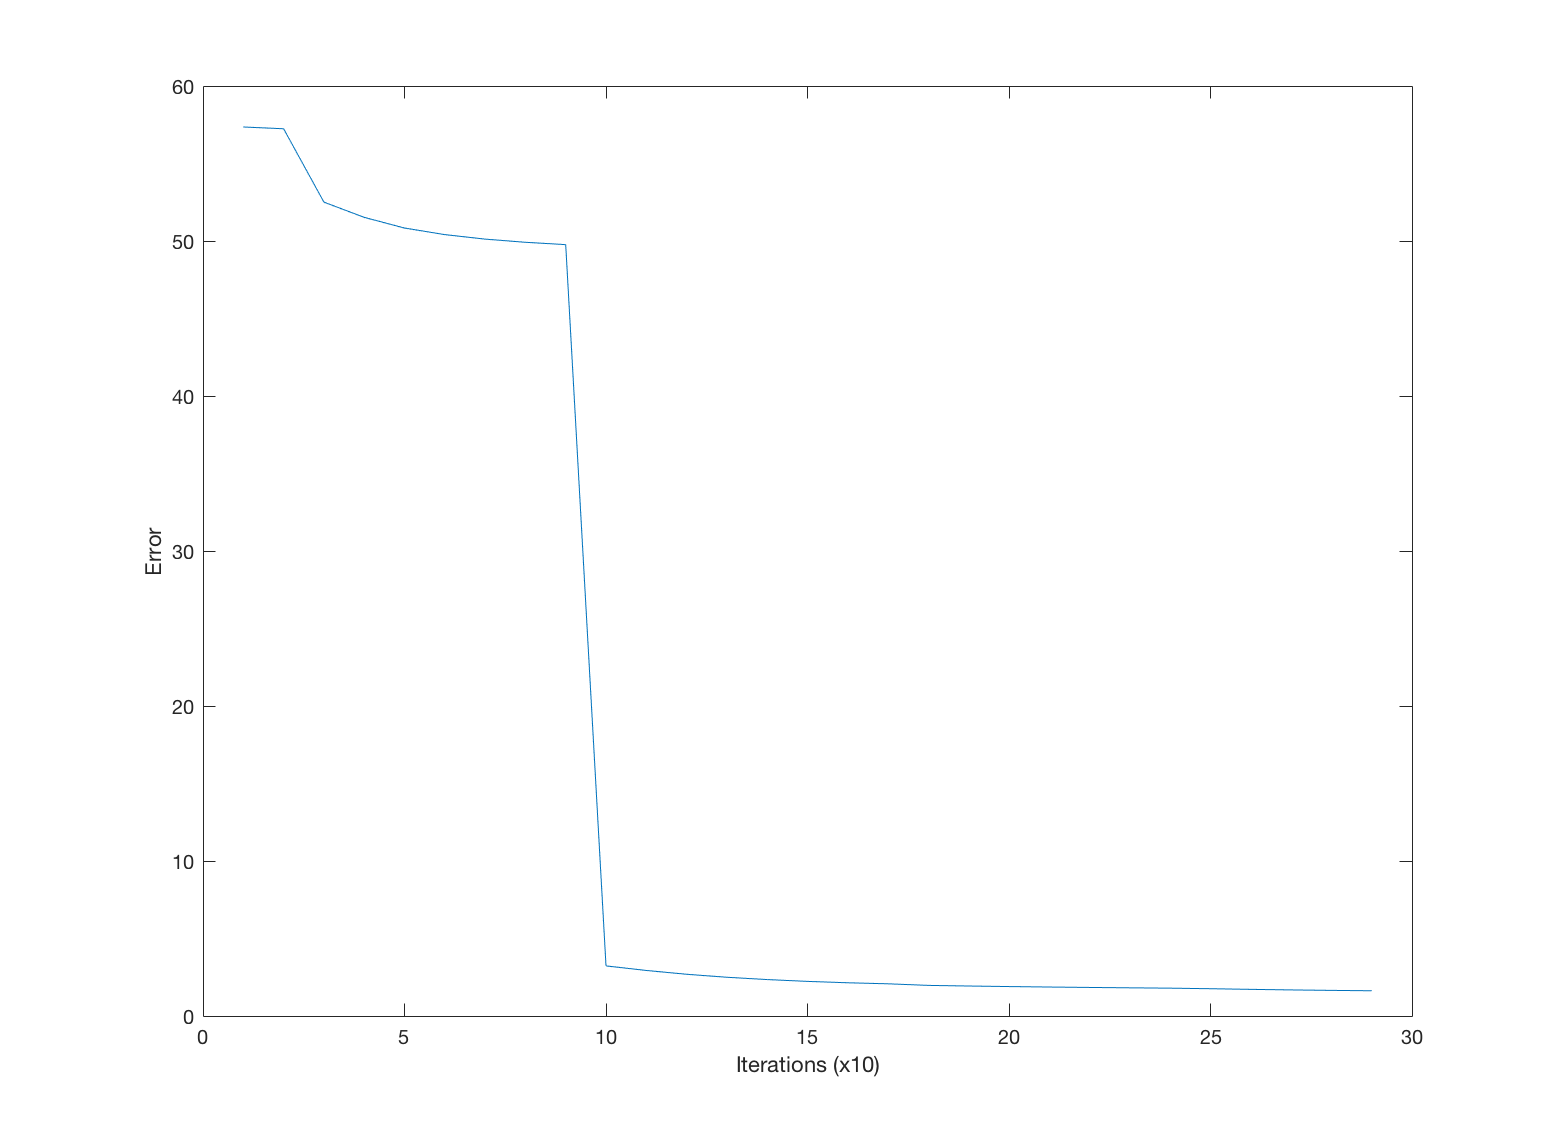
\includegraphics[width=\linewidth]{../../pracs/week6/images/q6_error}
    \centering
    \caption{Error vs Iteration\label{fig:q6}}
\end{figure}

\begin{figure}[H]
    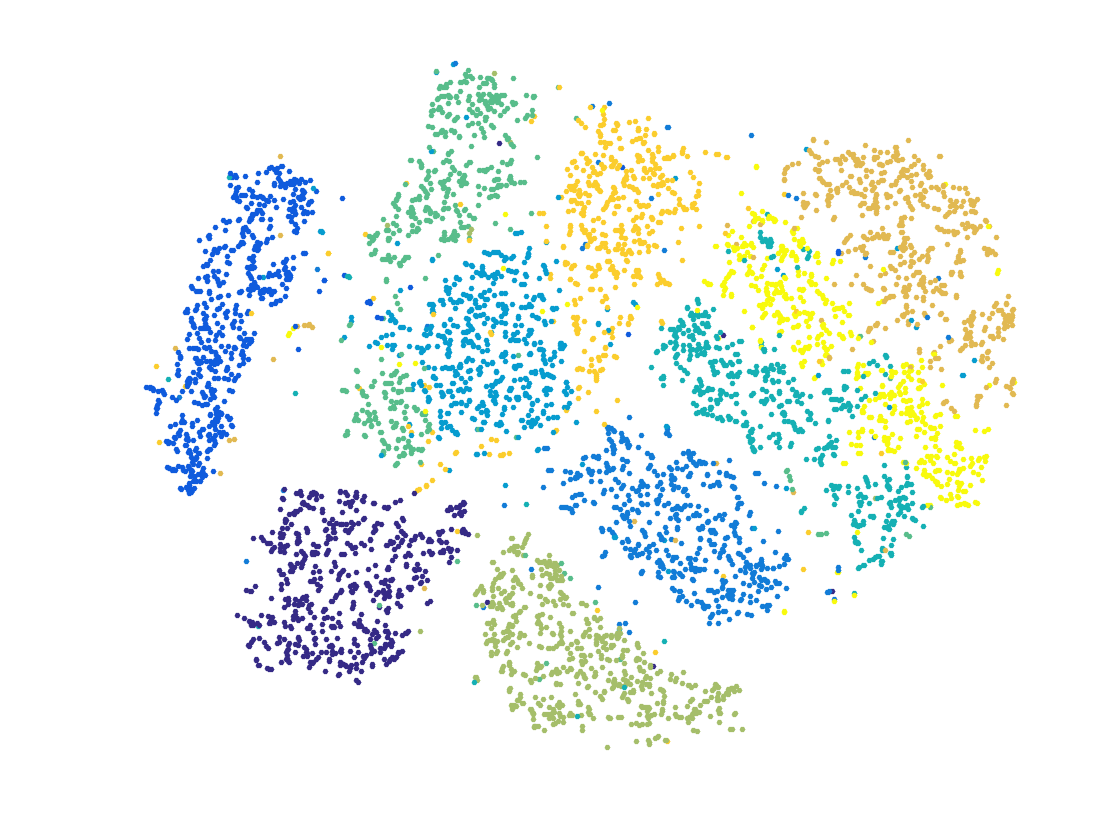
\includegraphics[width=\linewidth]{../../pracs/week6/images/q6}
    \centering
    \caption{Iteration 300\label{fig:tsne}}
\end{figure}

\section*{Question 5.8}

\begin{figure}[H]
    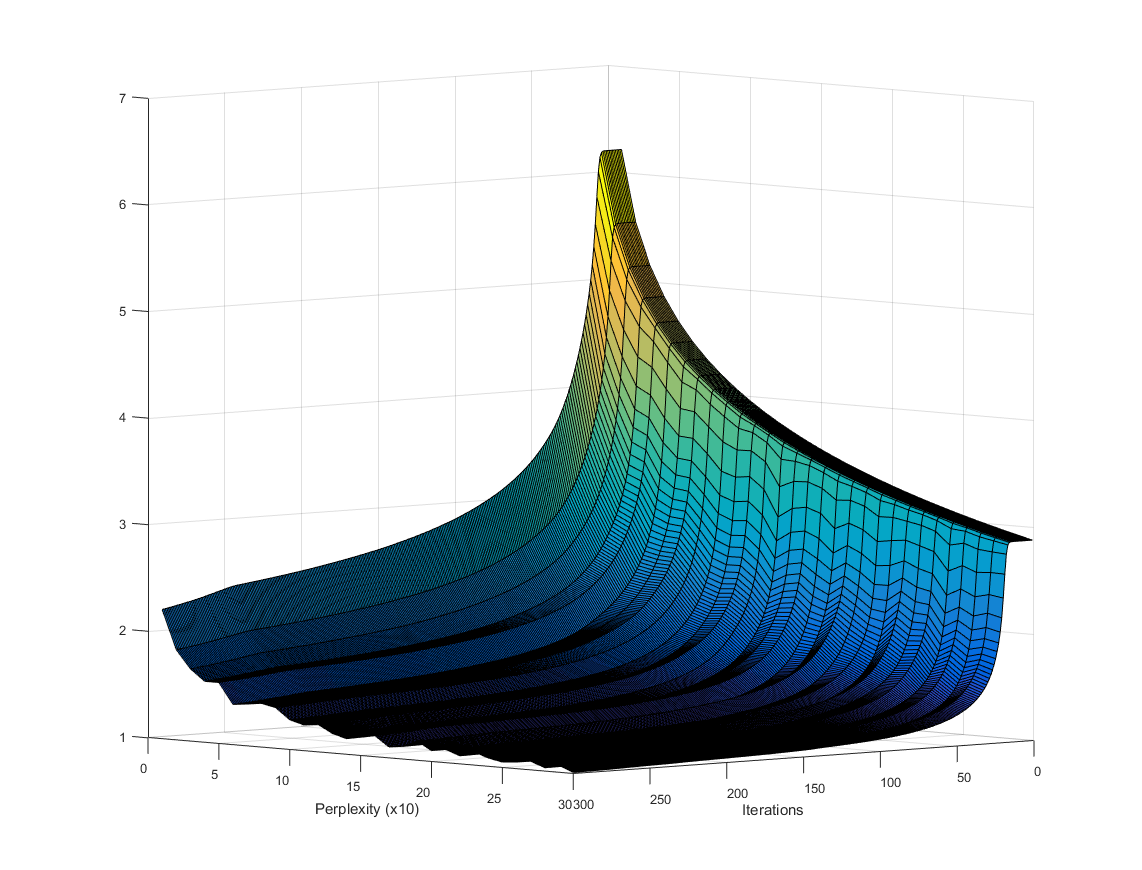
\includegraphics[width=\linewidth]{../../pracs/week6/images/q8}
    \centering
    \caption{Perplexity and Iterations on Cost}
\end{figure}

The above graph shows the perplexity and iterations on the cost (error).
From inspecting the graph it can be seen that increasing the iterations has a much larger effect than increasing the perplexity.
Thus it is clear that the number iterations has a much greater influence on the data than the perplexity.
Also its worth noting the graph shows a plateau when the number of iterations is small (when number of iterations is between 0 and 25).
Additionally after the plateau there is a steep fall in the error as the iterations increase,
with the error starting to flatten at the 100 iterations mark.
The perplexity determines how to balance the attention between local and global aspects of the dataset,
the original paper written on t-SNE suggests a value for the perplexity between 5 and 50\cite{ictdbid:2777}.
From the above graph it can be seen that the cost is highest with small values for iterations and perplexity, thus those low numbers are not suitable for the heuristic.

However as the perplexity and iterations increase, the error decreases.
Thus a valid heuristic would be to choose the largest number for perplexity and iterations as possible,
as this will guarantee a smaller error.
There is a trade off for this method as the number of iterations will increase the computation time.
Additionally perplexity should be less than the number of data points\cite{wattenberg2016how}.

\begin{figure}[H]
    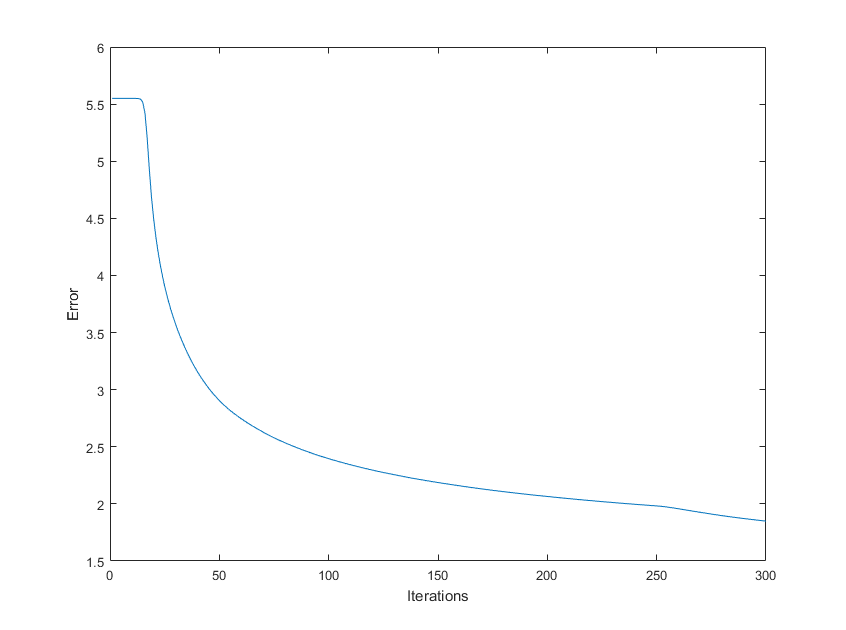
\includegraphics[width=\linewidth]{../../pracs/week6/images/q8_p2}
    \centering
    \caption{Error on iterations (perplexity = 2)\label{fig:2d_perp}}
\end{figure}

Figure~\ref{fig:2d_perp} shows a slice of the 3d graph when the perplexity is 2,
this illustrates the plateau from earlier and shows how the error flattens out when the number of iterations is increased.

% TODO: Talk about figure 13
%The graph shows the error change on iterations, thus we should choose a perplexity the reduces the error as quickly as possible, such that the algorithm requires less iterations to find a good solution.
%A simple heuristic to choose a good perplexity would be to look for the greatest rate of change in the error, by inspecting the chart we can see that the lower perplexities have far greater rate of change.
%Further inspection showed that a perplexity value of 2 provided the best rate of change.
% TODO: Write this

Figure~\ref{fig:2d_perp} differs from the figure~\ref{fig:q6} as the other chart as a large dip in the error at the 100 iteration mark.
This is because of the lines that were commented out, as those lines introduce a larger momentum that decays over each iteration. Line 87-89 of \verb|tsne_p.m| tells t-SNE to stop lying about the p-values when it reaches the 100th iteration, which explains the massive drop in error.

\begin{figure}[H]
    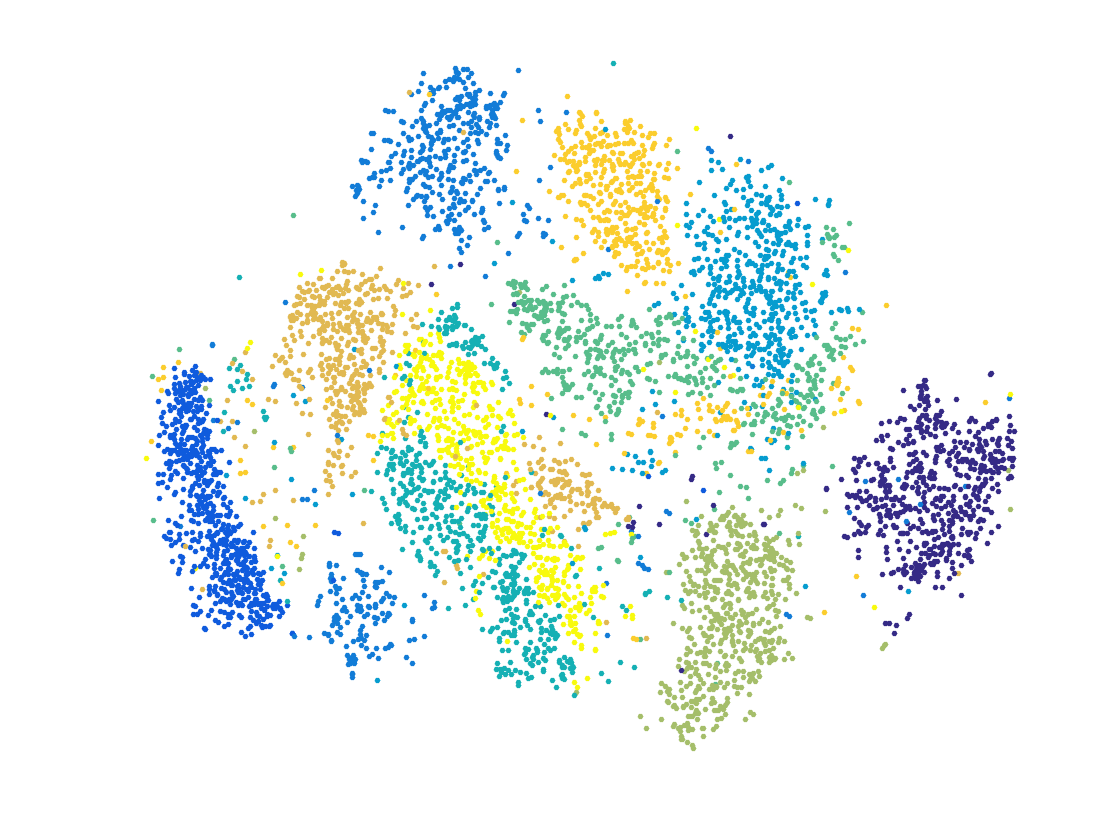
\includegraphics[width=\linewidth]{../../pracs/week6/images/tsne_large_perplexity}
    \centering
    \caption{TSNE at 300 iterations\label{fig:tsne2}}
\end{figure}

Figure~\ref{fig:tsne2} is similar to figure~\ref{fig:tsne}, however there are a few differences.
The major distance is the grouping of the classes, figure~\ref{fig:tsne} has much tighter grouping and better separation of classes,
however as figure~\ref{fig:tsne} has a lower perplexity, it could be attempting to cluster local minima.

\section*{Question 6.3}

Using the code generated from the \verb|nprtool|, the MNIST dataset can be easily loaded however there are various design choices that should be addressed.

The first design choice is the network training function, Matlab supports a lot of different training algorithms, such as gradient descent backpropagation, gradient descent with momentum and scaled gradient backpropagation.

I chose the scaled gradient backpropagation (\verb|trainscg|) function as it does not require a line search on each iteration,
which is described as a computationally intensive operation in the Matlab documentation.
The Matlab describes the downside of adopting this function is it takes more iterations to converge than the other algorithms,
but the speed increase is worth it.

% TODO: Talk about momentum

Another design parameter is the number of neurons in the hidden layers.
% TODO: Cite Scikit
The documentation for Scikit learn states the general rule of thumb for choosing values for the hidden layers is a value between the number of neurons in the input and output layers.
As we are dealing with 784 input layers and 10 output layers, any value between those would work.
To choose a suitable value, the network was trained against 15, 30, 45 and 60 hidden neurons, below is a chart showing the results.

\begin{figure}
  \begin{subfigure}[t]{.5\textwidth}
    \centering
	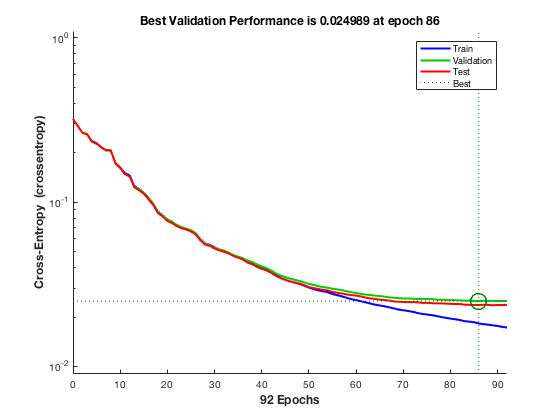
\includegraphics[width=\linewidth]{../../pracs/week7/images/15_hidden_neurons}
	\caption{15 hidden neurons training}
  \end{subfigure}
  \hfill
  \begin{subfigure}[t]{.5\textwidth}
    \centering
	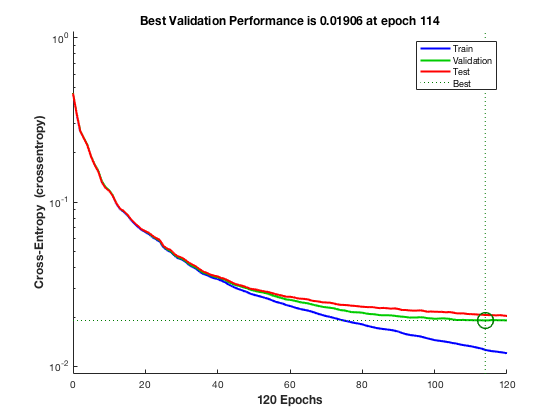
\includegraphics[width=\linewidth]{../../pracs/week7/images/30_hidden_neurons}
	\caption{30 hidden neurons training}
  \end{subfigure}

  \medskip

  \begin{subfigure}[t]{.5\textwidth}
    \centering
	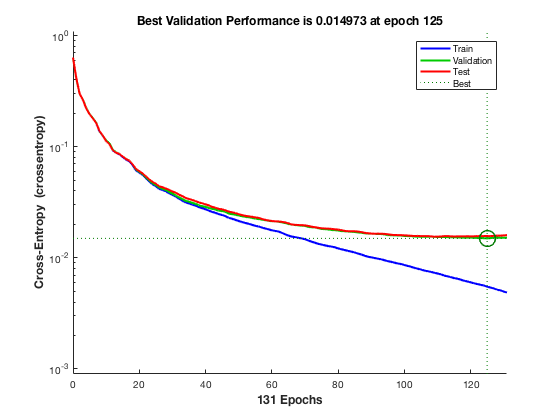
\includegraphics[width=\linewidth]{../../pracs/week7/images/45_hidden_neurons}
	\caption{45 hidden neurons training}
  \end{subfigure}
  \hfill
  \begin{subfigure}[t]{.5\textwidth}
    \centering
	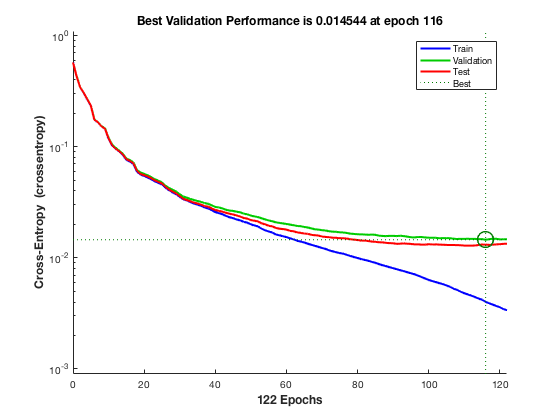
\includegraphics[width=\linewidth]{../../pracs/week7/images/60_hidden_neurons}
	\caption{60 hidden neurons training}
  \end{subfigure}
    \caption{Training results\label{fig:training_results}}
\end{figure}

The results of the training was summarised into the following graph.

\begin{figure}[H]
    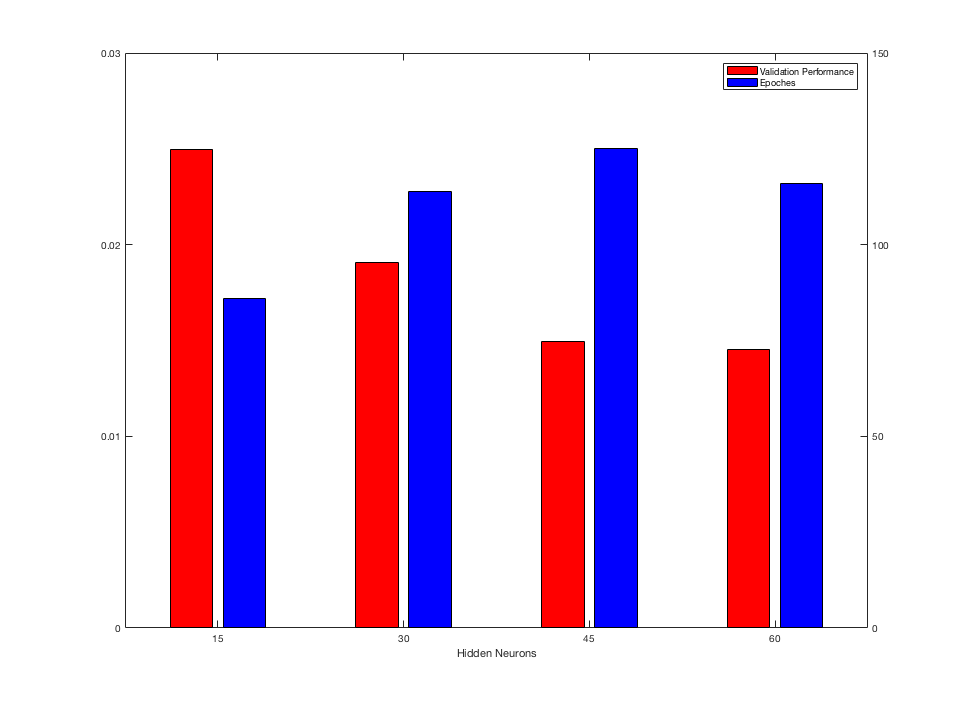
\includegraphics[width=0.7\linewidth]{../../pracs/week7/images/neurons_plot}
    \centering
    \caption{Number of Neurons vs Performance and Epochs}
\end{figure}

It can be seen that after 45 neurons, there are only marginal increases in performance, but the number of epochs until converging increases, thus increasing the running time of the program.
As a result 60 hidden layers was selected for the dataset.

\begin{figure}[H]
    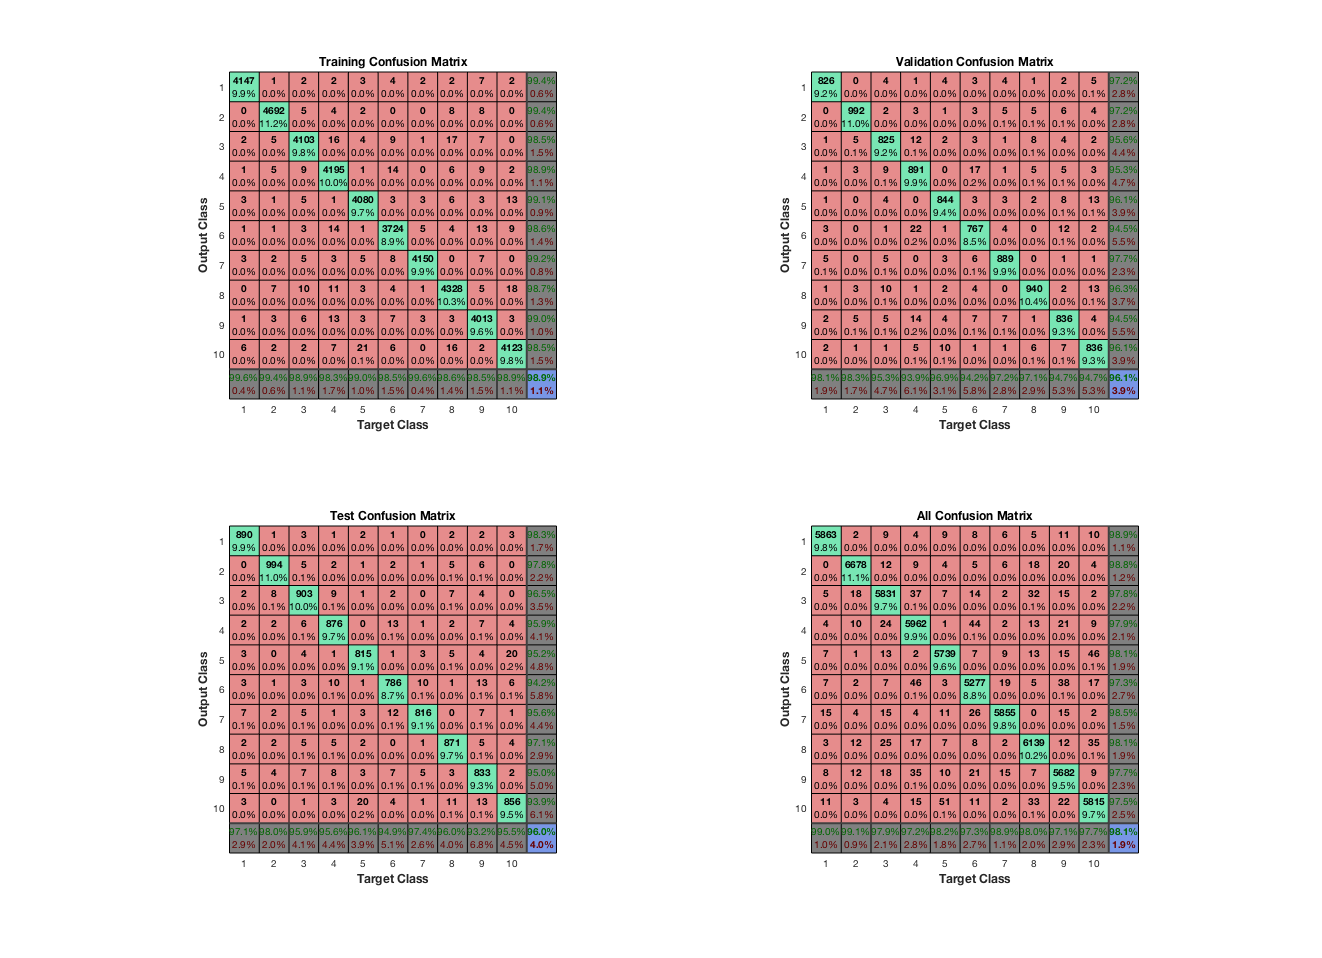
\includegraphics[width=\linewidth]{../../pracs/week7/images/60_hidden_neurons_confusion}
    \centering
    \caption{60 hidden neurons confusion matrix}
\end{figure}

The above confusion matrix chart shows the error in the algorithm.
The validation confusion matrix shows that the overall error is 3.9\%.

This can be compared to Figure 9 in the paper ``Gradient-Based Learning Applied to Document Recognition''\cite{lecun1998gradient}, which found the error rate to be 4.7\%. 

Its also worth noting the error on the training confusion matrix, which has by far the lowest error at 1.1\% which matches the blue line from part d in figure~\ref{fig:training_results}.

\bibliographystyle{unsrt}
\bibliography{references}

\end{document}
